\documentclass[tikz]{standalone}

\usetikzlibrary{decorations.pathmorphing,patterns}
\begin{document}
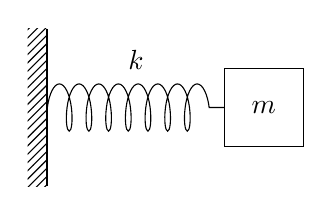
\begin{tikzpicture}
  %Roofs
  \fill [pattern = north east lines] (0,0) rectangle (0.25,2);
  \draw[thick] (0.25,0) -- (0.25,2);

  %Springs
  \draw[decoration={aspect=0.3, segment length=2.5mm, amplitude=3mm,coil},decorate] (0.25,1) -- (2.5,1) node at (1.375,1.5+0.1) {$k$};

  %Boxes
  \draw (2.5,0.5) rectangle (3.5,1.5);
  \node at (3,1) {$m$};

\end{tikzpicture}
\end{document}